% !TeX TS-program = xelatex
% !TeX root = template-UNAMFC.tex
% !TeX spellcheck = es_MX

\documentclass[spanish,11pt]{beamer}  %aspectratio=169

% ----------------------------------------------------- Font and input related
\usepackage[T1]{fontenc} 
\usepackage[utf8]{inputenc}
\usepackage[spanish]{babel} \spanishdecimal{.}


\usepackage{fontspec}       % XeLaTeX requre: Allow to use installed fonts
\usepackage{unicode-math}	% Allow to use other fonts in math mode
%	\setsansfont{Gotham}	% Beamer default font is sans: Needs Gotham in system
	\setsansfont{Booster Next FY}%{}
	\setmathfont{Latin Modern Roman} % Needs Lation Modern Roman in system
	\newfontfamily{\titlefont}{Gotham}%{Nimbus Sans}

\usepackage[table]{xcolor}
% This package 
%\usepackage[texcoord,grid,gridu	nit=mm,gridcolor=red!20,subgridcolor=green!40]{eso-pic}  

\usepackage{pdfpages}		
\geometry{papersize={280mm,157.5mm}}	% Convas is in 16:9 aspect ration 
										% and a 11pt fontsize in normal text works well 
\usepackage{setspace}
	\setlength{\parskip}{1em}
	\setlength{\parindent}{0em}
	\setlength{\itemsep}{2em}
\usepackage{multicol}						% for pages with multiple text columns, e.g. References
	\setlength{\columnsep}{10pt} 				% space between columns; default 10pt quite narrow
\usepackage{multirow}
\usepackage[margin=10pt,font=scriptsize,labelfont=bf]{caption}
\usepackage[labelformat=simple]{subcaption} 
\usepackage{float}
\renewcommand*{\thesubfigure}{\alph{subfigure})}
% ----------------------------------------------------- Math typesetting	
\usepackage{mathtools}
\usepackage{amsmath} 
\usepackage{physics}
\usepackage{bm}
\usepackage{bbm}
\usepackage{bbold}
\usepackage{listings}

% ----------------------------------------------------- Beamer optional packages
\usepackage[absolute,overlay]{textpos}		% Use of textes
\usepackage{appendixnumberbeamer}
\usepackage{svg}
\usepackage{fancyhdr}
\usepackage{pgfplots}
\usepackage{textcomp}


% tikz libraries
\usepackage{tikz}
\tikzset{>=latex} % for LaTeX arrow head

\usetikzlibrary{arrows.meta}
\usetikzlibrary{calc}
\usetikzlibrary{decorations.pathreplacing}
\usetikzlibrary{positioning}
\usetikzlibrary{shapes}

% pgfplots libraries
\usepgfplotslibrary{fillbetween}
% ----------------------------------------------------- References 
\usepackage[ bibstyle = trad-abbrv,
			citestyle = numeric-comp,
			backend = bibtex,
			maxcitenames=1,
			date = year,
			doi = false, 
			url = false,
			isbn = false
			]{biblatex}%trad-abbrv numeric-comp
	\DeclareFieldFormat[article]{volume}{\mkbibbold{#1}}
	\DeclareFieldFormat[article]{title}{}
	\AtEveryBibitem{\clearfield{month}}
	\AtEveryBibitem{\clearfield{day}}
	\DefineBibliographyStrings{spanish}{andothers = {et\addabbrvspace al\adddot}}
	\renewbibmacro*{journal}{%
		\ifboolexpr{ test {\ifcitation} and not test {\iffieldundef{shortjournal}}
		}
		{\printfield[journaltitle]{shortjournal}}
		{\iffieldundef{journaltitle}
			{}
			{\printtext[journaltitle]{%
				\printfield[titlecase]{journaltitle}%
				\setunit{\subtitlepunct}%
				\printfield[titlecase]{journalsubtitle}
									}
			}
		}
	}
\addbibresource{tex/references.bib}







		






\usepackage{lipsum}
\usetheme{UNAMFC}

%\graphicspath{{img}}

\title
    [Título corto]
    {Título de algo muy largo que se va a presentar en la Facultad de Ciencias}
\subtitle{Subtítulo de esa presentación} 
\author
    [\hyperlink{fr:Contenido}{J. A. Urrutia Anguiano}]
    {\emphb{Jonathan Alexis Urrutia Anguiano$^{1}$}\\
    {Nombre de colaboradores}}
\institute
    [Grupo de investigación]
    {Departamento de Física\\
    Facultad de Ciencias\\
    Universidad Nacional Autónoma de México
    }
\date
    [dd/mm/yy]{día de mes de año}

 
\titlegraphic{
	
\includegraphics[width = 110mm]{Latex/Logo_FC_Color.png}
  	}

\begin{document}

% -------------------------------------------------- Title with extra image
% ----------------------------- With no image you can simple use \maketitle
\begin{frame}\titlepage
  	\begin{beamercolorbox}{author}
    	  \usebeamerfont{institute}
    	  \hspace*{.5em}\large\emphb{$^1$}\url{jaurrutia.95@ciencias.unam.mx}
  	\end{beamercolorbox}\par
  \begin{textblock*}{75mm}(200mm, 120mm)
	
\includegraphics[width = 75mm]{Latex/pcf-logo.png}
  \end{textblock*}
\end{frame}

% -------------------------------------------------------- Table of contents
\begin{frame}{Contenido}
	\label{fr:Contenido}
	\tableofcontents
\end{frame}
	
	% !TeX root = ../template-UNAMFC.tex
\section{Estructuras útiles}
%----------------------------------------------------------------------------------
\begin{frame}{\underline{¿Ventajas de esta plantilla?}} % De esta forma se pone el subrayado
	{No se reescala nada}
	\centering
	\begin{columns}
		\column{.9\squeezethree}
		Se debe copmpilar en \emphb{Xelatex} y tener instalado Gotham en las fuentes del sistema
		{\fontseries{l}\titlefont\selectfont Algo así}
		{\titlefont Algo así}
		\begin{itemize}
			\item El aspectratio es 16:9
			\item El tamaño de la hoja no es el de beamer pero permite lo siguiente:
			\begin{itemize}
				\item La letra defalt es 11pt
				\item Reecalado sin deformar la imagen
				\begin{itemize}
					\item Ni las ecuaciones se hacen feas
					\item Y gráficas sin escala se ven como la de la derecha
				\end{itemize}
			\end{itemize}
		\end{itemize}
		\vskip3em
		En Latex/setup.tex está el paquete de \emphr{esp-grid}. Si se descomenta se muestran las coordenadas para colocar varios de los elementos en esta plantilla.
		
		\column{1.8\squeezethree} \centering
		Image with scale = 1 with a font of 11pt\\[1em]
		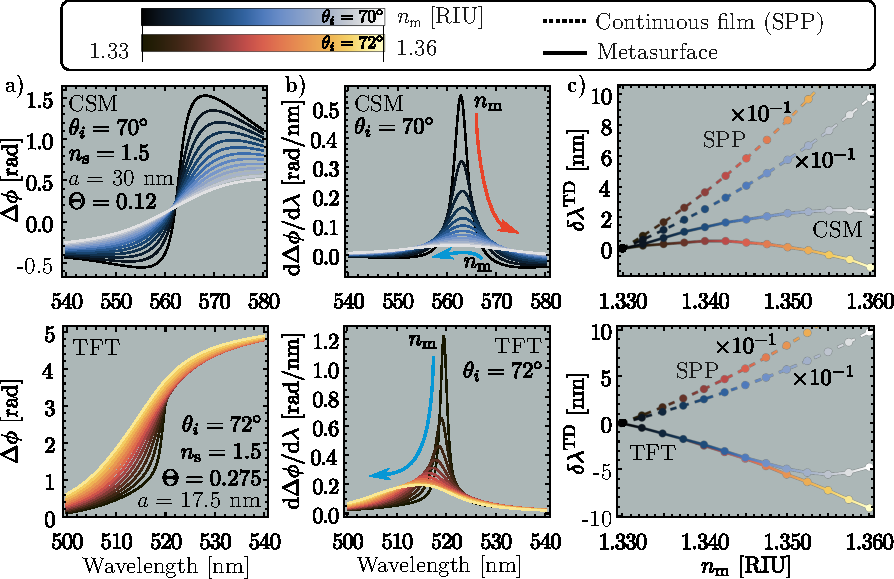
\includegraphics[scale = 1]{img/Fig-Sens.pdf}
	\end{columns}
	
\end{frame}

\section{Ejemplos de algunas diapositivas}
%----------------------------------------------------------------------------------
\begin{frame}[t]{\underline{Ejemplo de una diapositiva para el contexto}}
		{Beamercolorbox y tikz}

	\vskip2em%
	\hskip2em%
	\begin{beamercolorbox}[wd=\squeezethree]{}
		Pones el texto y \emphb{resaltamos algo} \emphr{con dos colores} y un a referencia a mano.\footnotemark[1]\\[1em]
    	
    	Una lista pequeña nada más
        \begin{itemize}  
            \item Parametro 1
			\item El 2
			\item Y el tercero
        \end{itemize}
    \end{beamercolorbox}%
     \begin{textblock*}{40mm}(50mm,60mm)\scriptsize
     	\rule{20mm}{.5pt}\\
    	\footnotemark\fullcite{gonzalez-alcalde_large_2020}
    \end{textblock*}

	
% Nanorods kabashin_plasmonic_2009 -------------------------------
    \begin{textblock*}{1mm}(105mm,20mm)
	\begin{tikzpicture}[font=\scriptsize]
	\node (img) {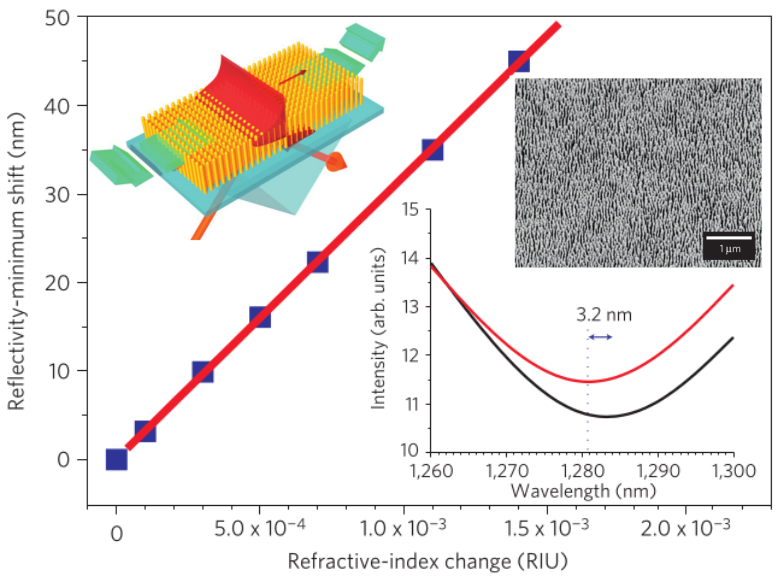
\includegraphics[width = 85mm]{img/1-nanorods.png}};
	\path (img.45) node [anchor = north west, xshift=10mm] {\begin{minipage}{30mm}
			\begin{flushleft}
                \fullcite{kabashin_plasmonic_2009} \\[1em]
				La referencia de la imagen se pone a mano\\[1em]
				Y se coloca relatiava a la imagen grande
			\end{flushleft}
			\end{minipage}};	
	\end{tikzpicture}
    \end{textblock*}



    % COVID qiu_dual_2020 -----------------------------------------
    \begin{textblock*}{1mm}(10mm,85mm)
	\begin{tikzpicture}[font=\scriptsize]
		\node (img) {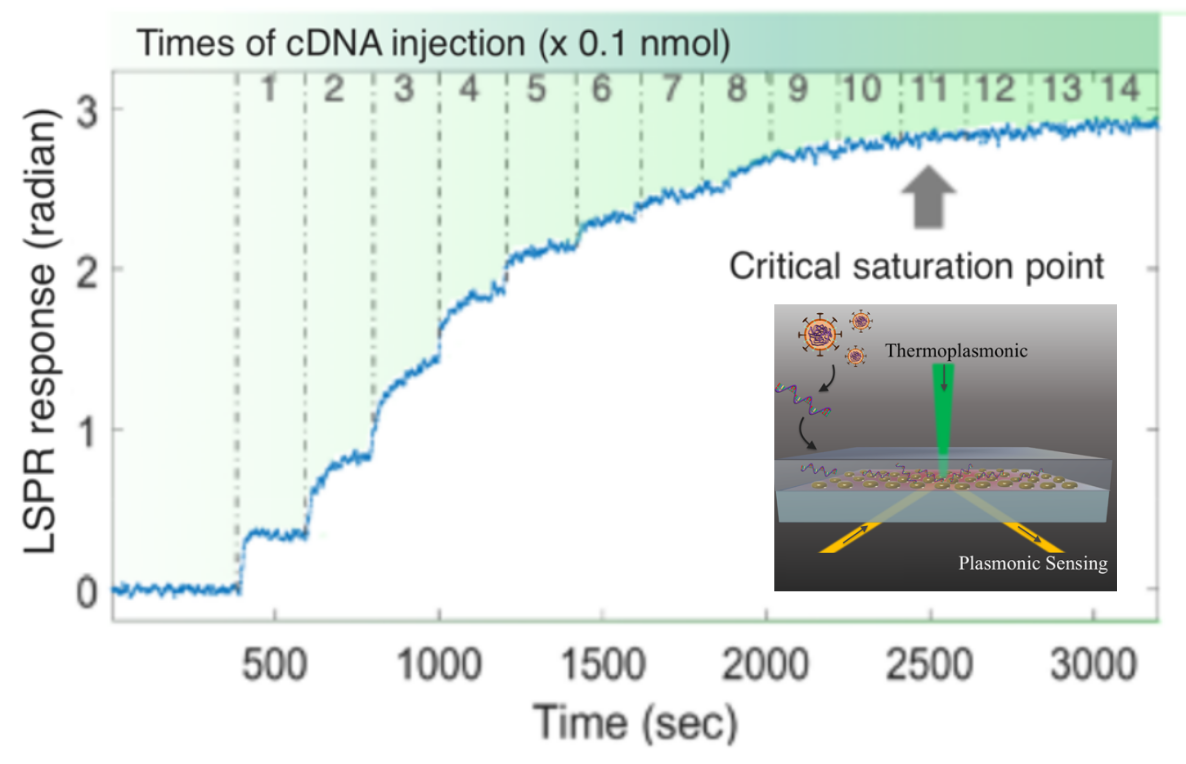
\includegraphics[width = 95mm]{img/1-covid.png}};
		\path (img.0) node [anchor = north west, xshift=-2.5mm] {\begin{minipage}{30mm}
				\begin{flushleft}
				\fullcite{qiu_dual_2020} \\[1em]
				Se usa flushleft\\
				flush   right\\
				Y textblock
				\end{flushleft}
		\end{minipage}};	
	\end{tikzpicture}
	\end{textblock*}


    % Nanodisks svedendahl_refractometric_2014 --------------------
    \begin{textblock*}{1mm}(170mm,65mm)
	\begin{tikzpicture}[font=\scriptsize]
		\node (img) {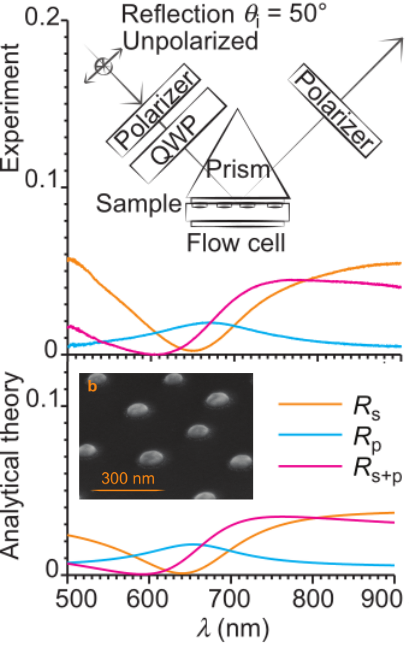
\includegraphics[width = 55mm]{img/1-phase.png}};
		\path (img.180) node [anchor = north east, xshift=0mm] {\begin{minipage}{30mm}
				\begin{flushright}
	                \fullcite{svedendahl_refractometric_2014}\\[1em] 
					Hay que entender como funciona
					node, ancho y  path en tikz.
				\end{flushright}
		\end{minipage}};	
	\end{tikzpicture}
\end{textblock*}
\end{frame}




	% !TeX root = template-UNAMFC.tex

\section{Tikz y Beamer}
	\subsection{Tikz}
		\subsubsection{Flowboxes}

\begin{frame}{Hablamos de nuestro proyecto}
	{\textoverline{Con metas parciales, referencias y  resaltando  lo que hacemos nosotros}}
%		{\rlap{Con metas parciales, referencias y  resaltando  lo que hacemos nosotros}\rule[1em]{\widthof{Con metas parciales, referencias y  resaltando  lo que hacemos nosotros}}{1.3pt}}
	
    \begin{center}
    \begin{tikzpicture}[node distance=15mm and 15mm,font=\normalfont]
%        \setlength{\leftmargini}{10pt}

    % caract
        \node[flowbox] (caract) {%
            \fbtitle{Caracterización}\vphantom{yÖ}
         \nodepart{two}
            \begin{minipage}{.17\textwidth}
                \begin{itemize}\itemsep0em
                    \item Experimental
                    \item Teórica
                    \item Numérica
                \end{itemize}
            \end{minipage}
        };

    % quiestion
        \node[concept,above=of caract,align=center,yshift=-.6cm] (question) {
            Metasuperficie  plasmónica  desordenada
            };

        \draw[conn] (question) -- (caract);

    % teo
        \node[flowbox,right=of caract,yshift=0cm,onslide=<2->{fb-highlight}] (teo) {%
            \fbtitle{Teórica}\vphantom{yÖ}
         \nodepart{two}
            \begin{minipage}{.24\textwidth}
                \textit{Coherent Scattering Model\footnotemark[1]}\centering
                \begin{itemize}\itemsep0em  \small
                    \item Teoría de esparcimiento
                    \item Polidispersidad en tamaño
                    \item Partículas esféricas
                \end{itemize}
            \end{minipage}
        };

        \draw[conn] (caract) -- (teo);

    % num
        \node[flowbox,right=of teo,onslide=<2->{fb-highlight},xshift=0cm] (num) {%
            \fbtitle{Numérica}\vphantom{yÖ}
         \nodepart{two}
            \begin{minipage}{.20\textwidth}
                Descenso de gradiente\footnotemark[2]
                \begin{itemize}\itemsep0em
                    \item Ajuste a modelos
                    \item Minimizar error
                \end{itemize}
            \end{minipage}
        };

        \draw[conn] (teo) -- (num);

    % exp
        \node[flowbox,below=of teo] (exp) {%
            \fbtitle{Experimental}\vphantom{yÖ}
         \nodepart{two}
            \begin{minipage}{.24\textwidth}
                \begin{itemize}\itemsep0pt
                    \item Síntesis
                    \item Microscopía
                    \item Arreglo experimental\footnotemark[3]
                \end{itemize}
            \end{minipage}
        };


        % concept text nodes
        \node[concept, below right=of num,align=center,xshift=-1cm] (assump) {Biosensor};

        \draw[hidden] (question.east) -|
                      node[above,text=sdgrayFC,font=\itshape\scriptsize,anchor=south east] {Optimización/Condiciones experimentales}
                      (assump.30);%

        % connections
        {%
             \draw[conn] (exp.north -| teo.290) --
                        node[right,anchor=west,text=sdgrayFC,font=\itshape\scriptsize] {
                        \begin{minipage}{2cm}
                            \begin{flushleft}
                            Muestra
                            \end{flushleft}
                        \end{minipage}
                        }
                        (teo.290);
            \draw[conn] (teo.250) --
                        node[left,anchor=east,text=sdgrayFC,font=\itshape\scriptsize] {
                        \begin{minipage}{2cm}
                            \begin{flushright}
                            Diseño
                            \end{flushright}
                        \end{minipage}
                        }
                        (exp.north -| teo.250);
        }
        \draw[conn] (caract.south) |-
                        node[below,near end,anchor=north,text=sdgrayFC,font=\itshape\scriptsize] {
                        \begin{minipage}{2cm}
                            \begin{flushright}
                            Colaboración\\ INAOE
                            \end{flushright}
                        \end{minipage}
                        }
                        (exp.west);
        \draw[conn] (exp) -|
                        node[below,near start,anchor=north,text=sdgrayFC,font=\itshape\scriptsize] {Mediciones ópticas}
                        (num);
        \draw[conn] (num.300) |-
                        node[below,near end,anchor=north ,text=sdgrayFC,font=\itshape\scriptsize] {
                        \begin{minipage}{2cm}
                            \begin{center}
                            Análisis\\ sensitividad
                            \end{center}
                        \end{minipage}
                        }
                        (assump.west);
    \end{tikzpicture}
    \end{center}

    \begin{textblock*}{85mm}(170mm,115mm)
        \begin{flushleft}
        \begin{spacing}{0}\scriptsize%\fontsize{4}{12} \selectfont \boosterfont
            \footnotemark[1]\fullcite{vazquez-estrada_optical_2014}\\
            \footnotemark[2]\fullcite{barzilai_two-point_1988}\\
            \footnotemark[3]\fullcite{cuanalo_sensitivity_2022}
        \end{spacing}
        \end{flushleft}
    \end{textblock*}
\end{frame}


{\setbeamertemplate{frametitle}[centertitle]{}
\begin{frame}{\underline{Plantilla con título centrado: centertitle}}
	{Vale la pena leer el código de tikz}
	
	\begin{center}
		\begin{tikzpicture}[node distance=5mm and 60mm,font=\normalsize]
			%        \setlength{\leftmargini}{10pt}
			
			% mono
			\path (0,2) node[concept,align=center] (modelo) {
				Modelo teórico
			};
			\node[below=of modelo, font = {\normalsize}] {%
				\begin{minipage}{1.5cm}
					$\begin{aligned}
						&\vec{x} \equiv \text{Parámetros}\\
						&f_i(\vec{x}) \equiv \text{Modelo}\\
					\end{aligned}$
				\end{minipage}
			};
			
			\path (0,-5) node[concept,align=center] (exp) {
				Resultado experimental
			};
			\node[below=of exp,yshift=0cm, font = {\normalsize}] {%
				\begin{minipage}{1.5cm}
					$\begin{aligned}
						y_i(\vec{x}) &\equiv \text{Medición}\\
					\end{aligned}$
				\end{minipage}
			};
			
			\node[below right = of modelo, concept,align=center,yshift=-.5cm] (error) {
				Error};
			
			\node[below =of error,font = {\normalsize}](min){
				$\begin{aligned}
					F(\vec{x}) = \frac{1}{N}\sum_{i=1}^N\qty(f_i(\vec{x})-y_i)^2
				\end{aligned}$
			};
			
			\draw[hidden] (modelo.east) -| (error.north) ;
			\draw[hidden] (exp.east) -| (min.south) ;
			
			\node[flowbox,fb-highlight,right =of error,xshift=0cm,font = {\normalsize}] (des) {%
				\fbtitle{Descenso de gradiente}\vphantom{yÖ}
				\nodepart{two}
				\begin{minipage}{3.2cm}\centering
					$\begin{aligned}
						\vec{x}_{\ell+1} = \vec{x}_\ell - \gamma \nabla F(\vec{x}_\ell)
					\end{aligned}$
				\end{minipage}
			};
			
			\draw[hidden] (error.east) -- (des)
			node[right,near start,text=sdgrayFC,font=\itshape\normalsize,anchor=south] {
				Minimización
			};
			
			\node[flowbox,below=of des,yshift=-30mm,font = {\normalsize}] (barzilai) {%
				\fbtitle{Método de dos pasos}\vphantom{yÖ}
				\nodepart{two}
				\begin{minipage}{75mm}\centering
					$\begin{aligned}
						\gamma_\ell = \frac{\qty(\vec{x}_{\ell} - \vec{x}_{\ell-1}) \cdot  \qty[\nabla F(\vec{x}_\ell)-\nabla F(\vec{x}_{\ell-1})]}
						{\norm{\nabla F(\vec{x}_\ell)-\nabla F(\vec{x}_{\ell-1})}^2}
					\end{aligned}$
				\end{minipage}
			};
			
			\draw[conn] (des) -- (barzilai);
		\end{tikzpicture}
	\end{center}
	
	
	\begin{textblock*}{30mm}(185mm,80mm)
		\begin{flushright}\scriptsize
			\fullcite{barzilai_two-point_1988}
		\end{flushright}
	\end{textblock*}
	
\end{frame}
}

	
	% !TeX root = template-UNAMFC.tex

\subsection{Beamer}
	\subsubsection{Blocks y Multicols}


% -------------------------------------------------------------------------------------------
{\setbeamertemplate{frametitle}[righttitle]{}
\begin{frame}{Bloques de distintas índoles\footnotemark[1]y righttitle}
				{\textoverline{Multicols para controlar tamaño  y otras cosas spongo}}
%
\centering
	\begin{columns}
		\column{\squeezethree}
		\centering
			\begin{block}{block:  Es más limpio}
				Para multicols se  definieron mitades y tercias
				\begin{itemize} \itemsep.5em
					\item \backslash{squeezetwo}
					\item \backslash{squeezethree}
					\item \backslash{loosethree}
				\end{itemize}
			\end{block}
		\column{1.5\squeezethree}
		
			\begin{exampleblock}{\centering exampleblock}
				El de colores más oscuros y letra azul
			    \begin{align*}
					\vb{E}^\text{exc}_k(\vb{r}) = & \vb{E}^\text{inc}(\vb{r}) + \sum_{\ell\neq k}^N \vb{E}^\text{ind}_\ell(\vb{r})\\
					\vb{E}^\text{ind}_\ell(\vb{r}) = & \int\dd^3 r' \mathbb{G}(\vb{r},\vb{r}') \times
					\int\dd^3 r''\mathbb{T}(\vb{r}'-\vb{r}_\ell,\vb{r}''-\vb{r}_\ell) \vb{E}_\ell^\text{exc}(\vb{r}'')\\
					\langle\vb{E}(\vb{r})\rangle = & \vb{E}^\text{inc}(\vb{r}) +  \sum_{\ell = 1}^N  \left(\prod_{k = 1}^N \int\dd^3 r_k \rho(\vb{R}) \vb{E}^\text{ind}_\ell(\vb{r})\right)
				\end{align*}
			\end{exampleblock}
	\end{columns}
\vskip1em
	\begin{columns}
		\column{.9\squeezetwo}
		\begin{alertblock}{\hfill alertblock}
			Colores claros y rojo para resaltar cosas
			\begin{align*}
				\langle \vb{E}_\ell^\text{exc}(\vb{r}'',\vb{R})\rangle_\ell =& \vb{E}^\text{inc}(\vb{r}'')
				+ \sum_{\substack{m =1 \\ m\neq \ell}}^N  \int\dd^3 r' \mathbb{G}(\vb{r}',\vb{r}'') \times \notag\\
				& \int\dd^3 r'''\int \dd^3 r_m \rho(\vb{r}_m) \mathbb{T}(\vb{r}'-\vb{r}_m,\vb{r}'''-\vb{r}_m) \langle \vb{E}_m^\text{exc}(\vb{r}'',\vb{R})\rangle_{\ell,m}
				\\
				\langle \vb{E}_m^\text{exc}(\vb{r}'',\vb{R})\rangle_{\ell,m},
				&= \prod_{\substack{n =1 \\ n\neq \ell,m}}^N  \int\dd^3 r_n \rho(\vb{R}|\vb{r}_\ell,\vb{r}_m) \vb{E}^\text{exc}_n(\vb{r}'')
			\end{align*}
		\end{alertblock}
		\column{.9\squeezetwo}
	\end{columns}	% 

%


    \begin{textblock*}{75mm}(180mm,80mm)
    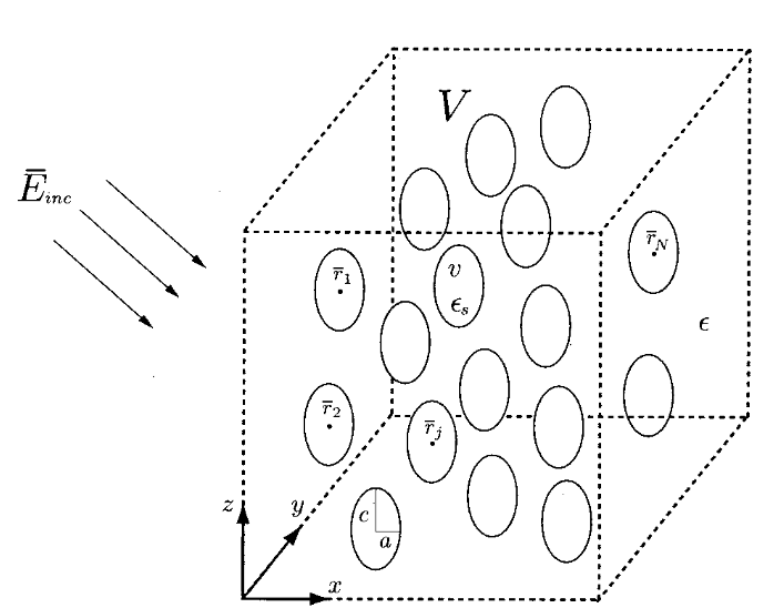
\includegraphics[width=75mm]{img/1-multiple.png}
\end{textblock*}
\begin{textblock*}{22mm}(175mm,120mm)
    \begin{flushright}
    \scriptsize
    \fullcite{ao_analytical_2002}
    \end{flushright}
\end{textblock*}


    \begin{textblock*}{80mm}(145mm,137.5mm)
        \begin{flushleft}
        \scriptsize
        \rule{30mm}{.5pt}\\
        \footnotemark[1]\fullcite{garcia2012multiple}
        Esto es un textlock aislado
    \end{flushleft}
     \end{textblock*}
\end{frame}
}

\begin{frame}{Título}{\textoverline{Subtítulo}}
	content...
\end{frame}
	

\end{document}

